% $Header: /Users/joseph/Library/texmf/tex/latex/beamer/solutions/conference-talks/conference-ornate-20min.en.tex,v 90e850259b8b 2007/01/28 20:48:30 tantau $

\documentclass{beamer}

% This file is a solution template for:

% - Talk at a conference/colloquium.
% - Talk length is about 20min.
% - Style is ornate.



% Copyright 2004 by Till Tantau <tantau@users.sourceforge.net>.
%
% In principle, this file can be redistributed and/or modified under
% the terms of the GNU Public License, version 2.
%
% However, this file is supposed to be a template to be modified
% for your own needs. For this reason, if you use this file as a
% template and not specifically distribute it as part of a another
% package/program, I grant the extra permission to freely copy and
% modify this file as you see fit and even to delete this copyright
% notice. 


\mode<presentation>
{
  \usetheme{Warsaw}
  % or ...

  \setbeamercovered{transparent}
  % or whatever (possibly just delete it)
}


\usepackage[polish]{babel}
% or whatever

\usepackage[utf8]{inputenc}
% or whatever

\usepackage{times}
\usepackage[T1]{fontenc}
% Or whatever. Note that the encoding and the font should match. If T1
% does not look nice, try deleting the line with the fontenc.


\title % (optional, use only with long paper titles)
{Automatyczna kompozycja kontrapunktu}

%\subtitle
%{Include Only ąęśćżźIf Paper Has a Subtitle}

\author % (optional, use only with lots of authors)
{Piotr Szachewicz}
% - Give the names in the same order as the appear in the paper.
% - Use the \inst{?} command only if the authors have different
%   affiliation.

%\institute[Universities of Somewhere and Elsewhere] % (optional, but mostly needed)
%{
%  \inst{1}%
%  Department of Computer Science\\
%  University of Somewhere
%  \and
%  \inst{2}%
%  Department of Theoretical Philosophy\\
%  University of Elsewhere}
% - Use the \inst command only if there are several affiliations.
% - Keep it simple, no one is interested in your street address.

%\date[CFP 2003] % (optional, should be abbreviation of conference name)
%{Conference on Fabulous Presentations, 2003}
% - Either use conference name or its abbreviation.
% - Not really informative to the audience, more for people (including
%   yourself) who are reading the slides online

%\subject{Theoretical Computer Science}
% This is only inserted into the PDF information catalog. Can be left
% out. 



% If you have a file called "university-logo-filename.xxx", where xxx
% is a graphic format that can be processed by latex or pdflatex,
% resp., then you can add a logo as follows:

% \pgfdeclareimage[height=0.5cm]{university-logo}{university-logo-filename}
% \logo{\pgfuseimage{university-logo}}



% Delete this, if you do not want the table of contents to pop up at
% the beginning of each subsection:
\AtBeginSubsection[]
{
  \begin{frame}<beamer>{Outline}
    \tableofcontents[currentsection,currentsubsection]
  \end{frame}
}


% If you wish to uncover everything in a step-wise fashion, uncomment
% the following command: 

%\beamerdefaultoverlayspecification{<+->}


\begin{document}

\begin{frame}
  \titlepage
\end{frame}

\begin{frame}{Plan}
  \tableofcontents
  % You might wish to add the option [pausesections]
\end{frame}


% Structuring a talk is a difficult task and the following structure
% may not be suitable. Here are some rules that apply for this
% solution: 

% - Exactly two or three sections (other than the summary).
% - At *most* three subsections per section.
% - Talk about 30s to 2min per frame. So there should be between about
%   15 and 30 frames, all told.

% - A conference audience is likely to know very little of what you
%   are going to talk about. So *simplify*!
% - In a 20min talk, getting the main ideas across is hard
%   enough. Leave out details, even if it means being less precise than
%   you think necessary.
% - If you omit details that are vital to the proof/implementation,
%   just say so once. Everybody will be happy with that.

\section{Cele projektu}

\begin{frame}{Co to jest kontrapunkt}
  % - A title should summarize the slide in an understandable fashion
  %   for anyone how does not follow everything on the slide itself.

  \begin{itemize}
  	\item kontrapunkt - dokomponowywanie melodii do danego głosu głównego.
  \end{itemize}
\end{frame}

\begin{frame}{Cel projektu}
	\begin{itemize}
		\item Wymyślenie i implementacja algorytmu do automatycznej kompozycji kontrapunktu gatunek I.
		\item Na podstawie: ,,Kontrapunkt. Podstawowe zasady.'', Gawlas J. 
	\end{itemize}

	\begin{figure}
	   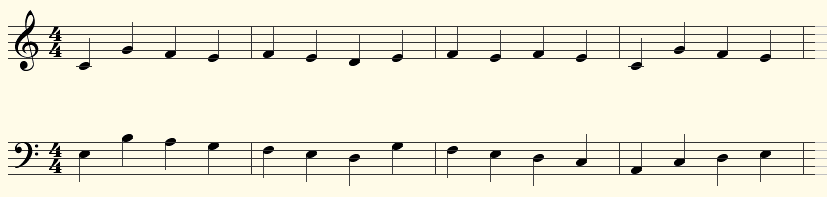
\includegraphics[scale=0.3]{nuty.png}
	\end{figure}
\end{frame}

\begin{frame}{Cel projektu}
	\begin{itemize}
		\item podstawowy przypadek użycia:
			\begin{itemize}
				\item Wprowadzenie melodii głosu głównego (wyklikanie myszką na pięciolinii)
				\item Wygenerowanie głosu kontrapunktującego przy pomocy algorytmu
				\item Wyświetlenie na pięciolinii wyniku (oba głosy)
			\end{itemize}
		\item dodatkowe możliwości:
			\begin{itemize}
				\item Możliwość odtworzenia wyniku
				\item Możliwość zapisania i wczytania wyniku lub głosu głównego z pliku
			\end{itemize}
	\end{itemize}
\end{frame}

\section{Logika}
\begin{frame}{Logika}
	Gatunek I:
	\begin{itemize}
		\item jednej nucie głosu głównego odpowiada jedna nuta głosu kontrapunktującego
 
	\end{itemize}
\end{frame}

\begin{frame}{Logika}
	Harmonia
	\begin{itemize}
		\item wszystkie współbrzmienia to konsonanse (1cz, 5cz, 8cz, 3m, 3w, 6m, 6w)
		\item rozpoczęcie i zakończenie to współbrzmienie konsonansu doskonałego (1cz, 5cz, 8cz)
		\item wszystkie wertykalne konsonanse doskonałe (1cz, 5cz, 8cz) muszą być osiągnięte ruchem 
		przeciwnym (oba głosy w przec. kierunkach) lub bocznych (jeden głos nieruchomy)
	\end{itemize}
\end{frame}

\begin{frame}{Logika}
	Melodia
	\begin{itemize}
		\item przeważają kroki (ruch o sekundę)
		\item przeważa ruch przeciwny (oba głosy w przeciwnych kierunkach)
		\item niedozwolone skoki melodii o: tryton, 7w, 7m.
	\end{itemize}
\end{frame}

\begin{frame}{Logika}
	Zasady swobodne
	\begin{itemize}
		\item mieszaj konsonanse doskonałe (1cz, 5cz, 8cz) i niedoskonałe (3, 6)
		\item unikaj 1cz w pierwszym i ostatnim współbrzmieniu
		\item unikaj skoku w obu głosach na raz
		\item po dużym skoku zmiana kierunku melodii i kroki sekundowe
		\item na przestrzeni 10-20 dźwięków głosu kontrapunktującego należy wykorzystać cały zakres skali
	\end{itemize}
\end{frame}

\begin{frame}{Liczba rozwiązań}

	Liczba możliwych rozwiązań:
	\begin{itemize}
		\item każda nuta może być w 1 z 7 odległości od głosu głównego (patrz. Harmonia)
		\item dla głosu głownego składającego się z N dźwięków jest $7^N$ różnych możliwości dopisania głosu kontrapunktującego
		\item Na przykład:
		\begin{itemize}
			\item $7^5 = 16807$
			\item $7^{10} = 282 475 249$
			\item $7^{15} = 4 747 561 509 943$
		\end{itemize}
	\end{itemize}
\end{frame}

\section{Technologie}
\begin{frame}{Technologie}
	\begin{itemize}
		\item Java
		\item Swing
		\item JMusic library – biblioteka do programowania muzyki (struktury danych, wizualizacja) z otwartym kodem źródłowym
		\item MIDI
	\end{itemize}
\end{frame}

\end{document}


